\documentclass{article}
 
%Russian-specific packages
%--------------------------------------
\usepackage[T2A]{fontenc}
\usepackage[utf8]{inputenc}
\usepackage[russian]{babel}
\documentclass[border=0.125cm]{standalone}
\usepackage{tikz}
\usetikzlibrary{positioning}
\usepackage{amsmath}
\usepackage{graphicx} %package to manage images
\graphicspath{ {./images/} }
%--------------------------------------
 
%Hyphenation rules
%--------------------------------------
\usepackage{hyphenat}
\hyphenation{ма-те-ма-ти-ка вос-ста-нав-ли-вать}
%--------------------------------------
 
\title{Распознаване рукописных образов цифр на основе сверточных нейронных сетей}
\author{Сиражетдинов Руслан ФТ-401}
 
\begin{document}
\maketitle
\newpage

\tableofcontents
\newpage

\section{Введение}
Распознование изображений компьютером является задачей компьютерного зрения и является актуальной в наше время цифровизации и автоматизации различных процессов. Одной из таких задач является распознование рукописных записей, для её решения можно применять различные алгоритмы, в том числе и нейронные сети, которые широко распространены, применяются и очень хорошо справляются с обработкой и классификацией изображений.

Для решения задач этой области применяются различные технологии, одним из удобных инструментом для реализации поставленных задач является \verb|MatLab| - пакет прикладных программ для технических вычислений и создания графических интерфесов.

\verb|MatLab| для рещения задачи классификации был выбран ввиду того, что по приложению существует большое колличество документации и есть возможность установки доплнительных пакетов специфичных для этой области.
\newpage


\section{Архитектура проекта}
Проект состоит из трёх частей
\begin{itemize}
  \item Реестр данных для обучения - набор изображений с цифрами
  \item Сверточная нейронная сеть - модель классификатора
  \item Графический интерфейс - для ввода и вывода данных пользователя
\end{itemize}
\newpage


\section{Модель классификатора}
Классификатор представляет собой сверточную нейронную сеть.
Работа свёрточной нейронной сети обычно интерпретируется как переход от конкретных особенностей изображения к более абстрактным деталям, и далее к ещё более абстрактным деталям вплоть до выделения понятий высокого уровня. Поэтому такой подход очень удобно использовать для распознования образов.

Рассмотрим слои нейронной сети

\begin{itemize}
  \item Входной слой - принимающий матрицу изображения 28 на 28 пикселей
  \item Сверточный слой - 20 сверток с фильтрующим размером 5х5
  \begin{SCfigure}
  \newline
	\centering
	\begin{tikzpicture}
		\node at (1.5,4){\begin{tabular}{c}Входное изображение\\\end{tabular}};
	
		\draw (0,0) -- (3,0) -- (3,3) -- (0,3) -- (0,0);
		
		\draw (2,2) -- (2.5,2) -- (2.5,2.5) -- (2,2.5) -- (2,2);
		\draw (2,0.5) -- (2.5,0.5) -- (2.5,1) -- (2,1) -- (2,0.5);
		\draw (1,1) -- (1.5,1) -- (1.5,1.5) -- (1,1.5) -- (1,1);
		
		\draw (2.5,2) -- (7,3.25);
		\draw (2.5,2.5) -- (7,3.25);
 
		\draw (2.5,1) -- (5.75,0.25);
		\draw (2.5,0.5) -- (5.75,0.25);
		
		\draw (1.5,1.5) -- (5.5,1.25);
		\draw (1.5,1) -- (5.5,1.25);
		
		\node at (5.75,4){\begin{tabular}{c}выходные свертки\end{tabular}};
		
		\draw[fill=black,opacity=0.2,draw=black] (5.5,1.5) -- (7.5,1.5) -- (7.5,3.5) -- (5.5,3.5) -- (5.5,1.5);
		\draw[fill=black,opacity=0.2,draw=black] (5,1) -- (7,1) -- (7,3) -- (5,3) -- (5,1);
		\draw[fill=black,opacity=0.2,draw=black] (4.5,0.5) -- (6.5,0.5) -- (6.5,2.5) -- (4.5,2.5) -- (4.5,0.5);
		\draw[fill=black,opacity=0.2,draw=black] (4,0) -- (6,0) -- (6,2) -- (4,2) -- (4,0);
	\end{tikzpicture}
	\label{fig:convolutional-layer}
\end{SCfigure}

  
  \item Слой пакетной нормализации - ускоряет вычисления с помощью обработки пачками.
  \item ReLU Слой - функция активации, выдает взвешенную сумму на нейроне.
  \begin{equation}
    Relu(x) & = max(0,x) \\
  \end{equation}

    \newpage
  \item Полносвязный слой - сеть из нейронов для учета всех признаков
  \tikzset{%
   neuron missing/.style={
    draw=none, 
    scale=2,
    text height=0.333cm,
    execute at begin node=\color{black}$\vdots$
  },
}

\begin{tikzpicture}[x=1.5cm, y=1.5cm, >=stealth]

\foreach \m/\l [count=\y] in {1,2,3}
{
 \node [circle,fill=black!50,minimum size=0.5cm] (input-\m) at (0,2.5-\y) {};
}
\foreach \m/\l [count=\y] in {4}
{
 \node [circle,fill=black!50,minimum size=0.5cm] (input-\m) at (0,-2.5) {};
}
 
 \node [neuron missing]  at (0,-1.5) {};
 

\foreach \m [count=\y] in {1}
  \node [circle,fill=black!50,minimum size=0.5cm] (hidden-\m) at (2,0.75) {};
  
\foreach \m [count=\y] in {2}
  \node [circle,fill=black!50,minimum size=0.5cm] (hidden-\m) at (2,-1.85) {};
  
 \node [neuron missing]  at (2,-0.3) {};


\foreach \m [count=\y] in {1}
  \node [circle,fill=black!50,minimum size=0.5cm] (output-\m) at (4,1.5-\y) {};
  
\foreach \m [count=\y] in {2}
  \node [circle,fill=black!50,minimum size=0.5cm] (output-\m) at (4,-0.5-\y) {};

 \node [neuron missing]  at (4,-0.4) {};

\foreach \l [count=\i] in {1,2,3,20}
  \draw [<-] (input-\i) -- ++(-1,0)
    node [above, midway] {$I_{\l}$};

\foreach \l [count=\i] in {1,16}
  \node [above] at (hidden-\i.north) {$H_{\l}$};

\foreach \l [count=\i] in {1,10}
  \draw [->] (output-\i) -- ++(1,0)
    node [above, midway] {$O_{ \l}$};

\foreach \i in {1,...,4}
  \foreach \j in {1,...,2}
    \draw [->] (input-\i) -- (hidden-\j);

\foreach \i in {1,...,2}
  \foreach \j in {1,...,2}
    \draw [->] (hidden-\i) -- (output-\j);

\foreach \l [count=\x from 0] in {Входной, Скрытый, Выходной}
  \node [align=center, above] at (\x*2,2) {\l \\ слой};
\end{tikzpicture}

  \item Слой Softmax - на выходе вектор вероятностей пренадлежности классу
  \begin{equation}
  softmax(x)_i = \frac{exp(x_i)}{\sum_{j}^{ }exp(x_j))}\\
  \end{equation}
  \item Классификационный слой - по вектору из вероятностей возвращает цифру
\end{itemize}
\newpage

\section{Обучение модели}
Для обучения нейронной сети были использованые размеченные (пронумерованные) данные с изображениями цифр

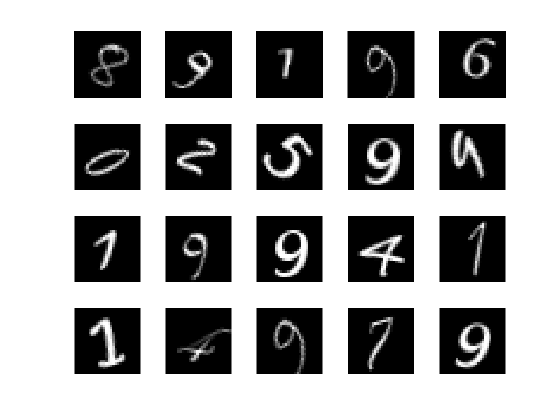
\includegraphics[scale=0.5]{numbers}

Обучение происходило со следующими гипер параметрами - 4 эпохи по 750 тренировочных подходов
Для проверки качества модель была проверена на валидационной выборке 

Метрика accuracy показала 90\% 
\newpage

\section{Создание графического интерфейса}
Графический интерфейс представляет собой панель для ввода произвольной графики слева и вывода классификации справа.

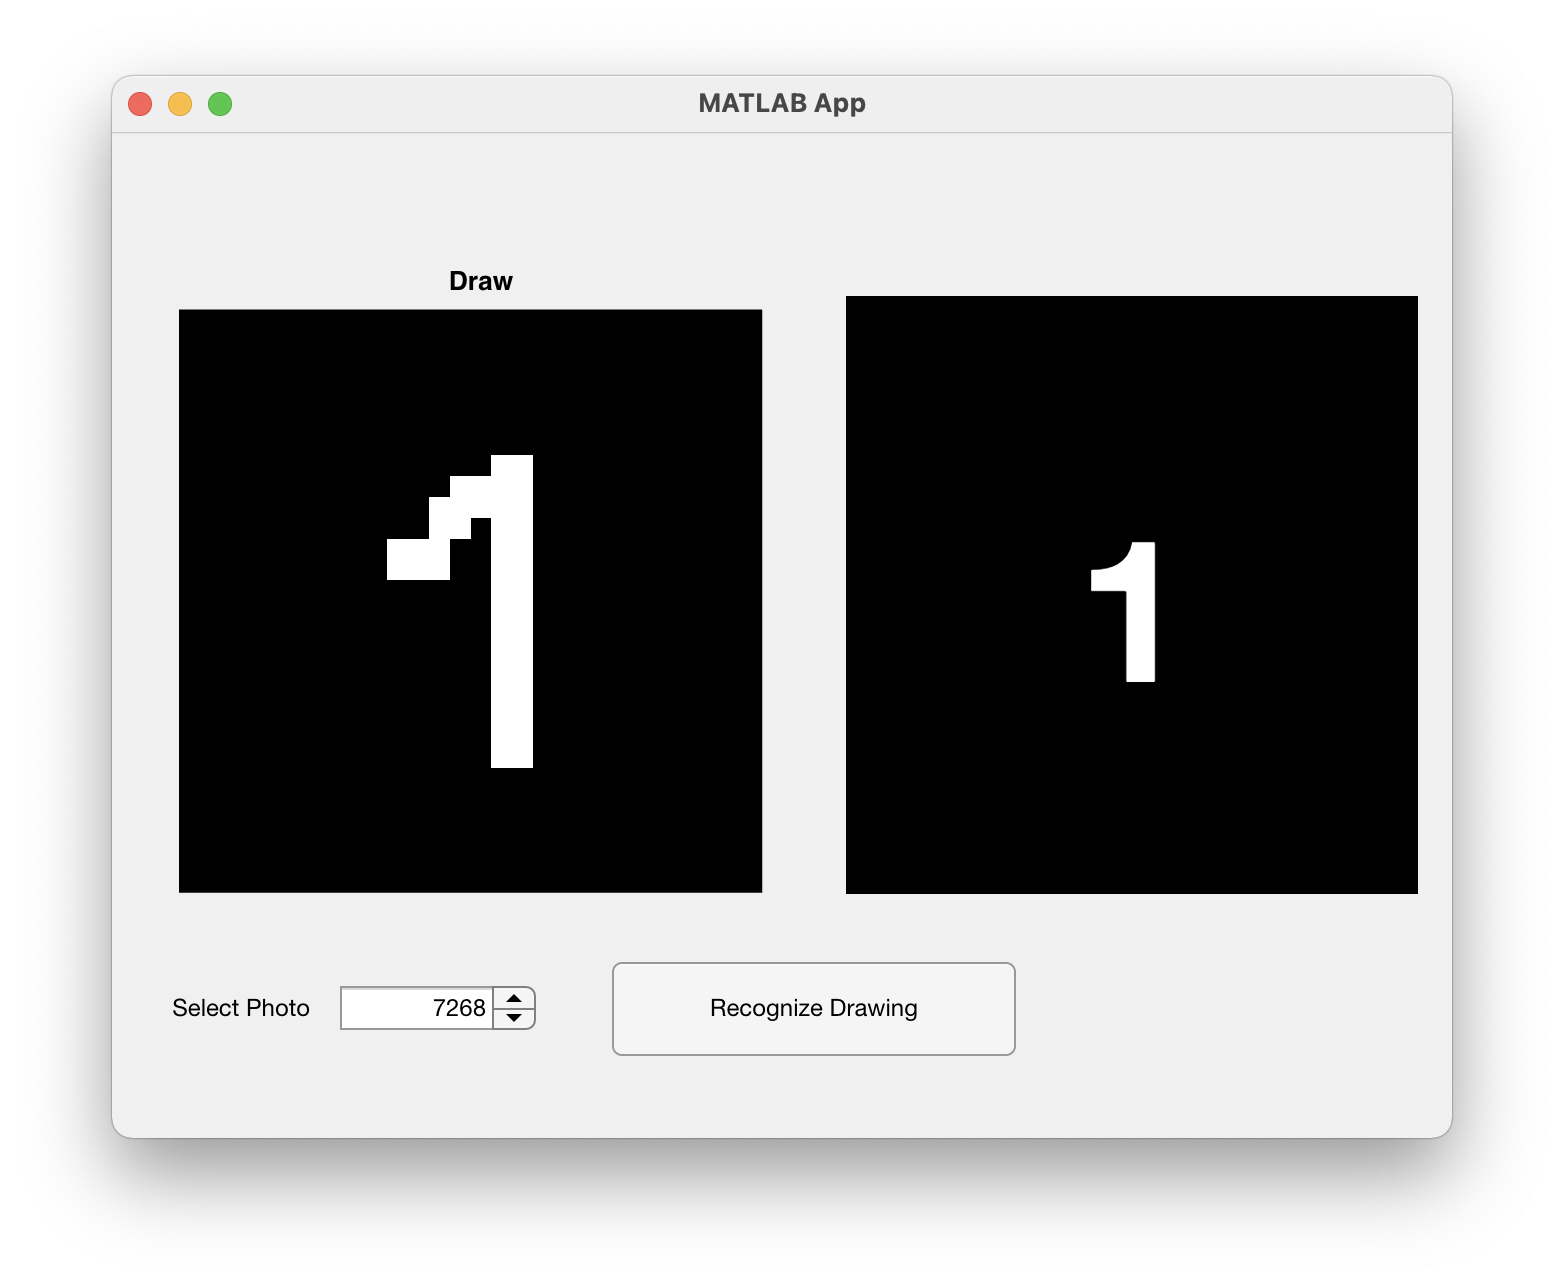
\includegraphics[scale=0.4]{app}

при запуске приложения в первый раз запустится обучение модели, что займет определенное колличество времени, по завершению обучения, модель сохранится на диск и повтороный запуск уже не потребует обучения.
\newpage 

\section{Заключение}
Мною было поэтапно реализовано приложение по распознаванию рукописных образов цифр. Для решения задачи я изучил различные сферы наук, такие как машинное обучение, анализ данных и разработка пользовательских интерфейсов.

Задача была декомпозирована на отдельные сущности: модель, реестр данных и интерфейс ввода-вывода. Такой подход позволит переиспользовать сущности в будущем в других проектах.

\begin{thebibliography}{3}
\bibitem{DeepLearning}
Ian Goodfellow, Yoshua Bengio, Aaron Courville  Deep Learning // Adaptive Computation and Machine Learning series --- P. 179--196.
\bibitem{UI}
Алан купер Интерфейс. Основы проектирования взаимодействия. 4-е изд. --- Издательский дом «Питер» --- 2016. --- 449 p.
\end{thebibliography}
 

\end{document}